\section{Overview}
\label{sec:overview}

% \begin{comment}
\begin{figure*}[h]
\centering
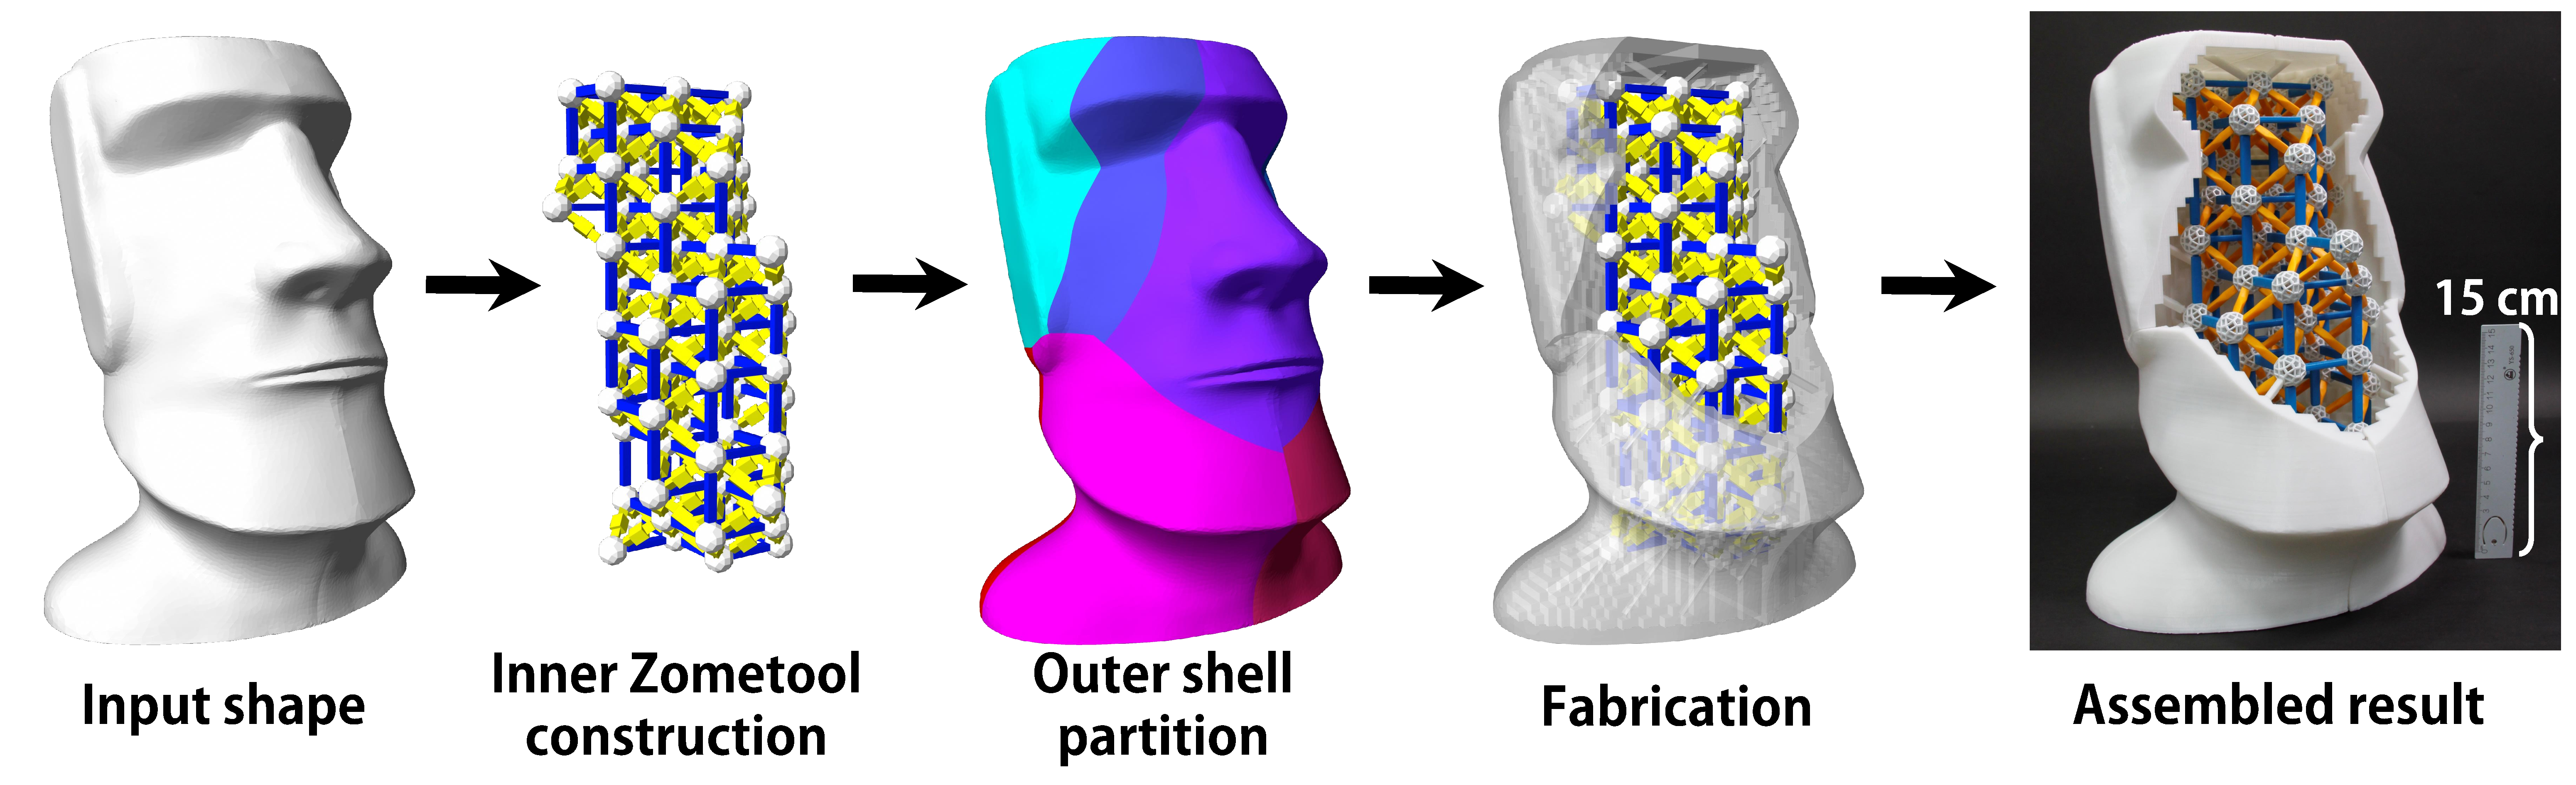
\includegraphics[width=1.0\linewidth]{figs/pipeline2.pdf} 
\caption{
Given input shape, we first optimize the inner Zometool structure (\secname~\ref{sec:Zometool}). Guided by optimized Zometool structure, we partition the outer shell (\secname~\ref{sec:surf_part}) and generate connectors for assembling both structures (\secname~\ref{sec:fab}).
The final fabricated result is obtained by assembling both assembled Zometool structure and printed outer shell.
}
\label{fig:result-pipeline}
\end{figure*}
% \end{comment}

Given a 3D shape, our method automatically generate\chinky{s} inner Zometool structure and outer 3D-printed shells.
% Zomefab is a method which combines Zometool and 3{D} printing for large-scale fabrication. 
Our method has the following features:
\begin{enumerate}
\item \textbf{Large Object.} Our method aim\chinky{s} for fabricating the large-scale object which it's height is from 0.3 to 1 meters, which is way larger than the printing volume of \chireplace{common}{ordinary} consumer-level 3{D} printer.
\item \textbf{Fabricability.} Each segment of the outer shell can be printed and fitted inside the volume of consumer-level 3{D} printer\chinky{s}.
\item \textbf{Assemblability.} The inner Zometool structure can be easily assembled and connected to the outer printed shells using \chireplace{special}{especially} designed connectors.
% 3{D} printing segments can assemble onto the inner structure.
\item \textbf{Cost-effectiveness.} Our method maximize\chinky{s} the inner structure and minimize the printing materials. 
It decreases the fabrication time and the cost of materials.
\end{enumerate}

\chireplace{Our method is illustrated in~\figname~\ref{fig:result-pipeline}.}{\figname~\ref{fig:result-pipeline} illustrates our method.}
% There is a flow chart at \figname~\ref{fig:result-pipeline}.
Given the input shape, we voxelize the inner volume of the input mesh to get the result of \chinky{an} initial Zometool structure.
Our goal is to grow the Zometool structure to occupied the maximum inner volume \chireplace{in order}{} to reduce most of the printing materials.
% get the maximum inner structure, but the structure of initial guess is too far from surface. 
Therefore, we design an optimization framework using simulated annealing, and design several local operations to explore the feasible Zometool structure space.
After the optimization, we get the maximum inner structure (\secname~\ref{sec:Zometool}).

Next, in order to print the outer shell of input shape, we have to (i) partition the shape into pieces where each piece can be fitted into printing volume, (ii) put connectors at feasible locations so that the inner Zometool structure and the outer shells can be connected robustly, and (iii) keep the salient region\chinky{s} intact.
We formulate the partition problem as \chireplace{a}{an} MRF problem and solve it with graph cut algorithm.
The intuition of this formulation is that each triangle should be connected to it's closest Zomeball, but simultaneously we want to reduce the number of partitions and maintain the integrity of salient region.
To further regularize the resulted partitions, we apply the SVM algorithm to find the hyperplane  between different labels and also use the hyperplane for our cut-plane to separate the mesh ( \secname~\ref{sec:surf_part}).
% we assign the triangle to it's nearest Zome-ball, but the number of labels is too much. 
% Hence, we use graph cut algorithm to help us optimize the classification and get the suitable number of labels. After the classification, we use Support Vector Machine classifier find the hyperplane between different labels and also use the hyperplane for our cut-plane to separate the mesh. (see \secname~\ref{sec:surf_part})

Last, before we separate the mesh by our cut-plane, we generate the inner surface by voxelizing the inner volume, and combine with the outer mesh as the solid mesh. 
% We voxelize inner volume of original mesh, and combine the result of voxelization, also the original mesh will become the new mesh. 
Then, we apply all cut planes on the solid\ignore{new }mesh and get the separate pieces. 
% But so far we just have the pieces, so 
We design the special connector and connect the pieces to the inner Zometool structure. 
Finally, the pieces with connectors can be printed and assembled to get the final large-scale object (\secname~\ref{sec:fab}).
% user gets the pieces with connector and assemble all of pieces to the inner structure, so that we can get the large-scale object by our method (\secname~\ref{sec:fab}).